\Chapter{THE APPROACH AND STUDY DEFINITION}\label{sec:Theme1}

%TOTAL = 15 pages

\section{The Approach}

%2 pages

This section will describe the steps followed to design \ac{TEDIOUS}, our proposed machine learning detector to identify design technical debts to self-admit. It will also define its characteristics, how it works and how to use it. \ac{TEDIOUS} works at method-level since it is typically the granularity at which developers introduce \ac{SATD} \citep{MaldonadoS15,PotdarS14}. In other terms, it is able to detect whether a method contains a design technical debt or not. Class-level granularity would be too coarse because technical debts normally admitted by developers are related to specific and punctual issues in the source code. Additionally, a class could contain a \ac{TD} but it would be impossible to precisely identify the source of the problem since a class contains several methods and \ac{LOC}. \par 

\begin{figure}[t]
	\centering
	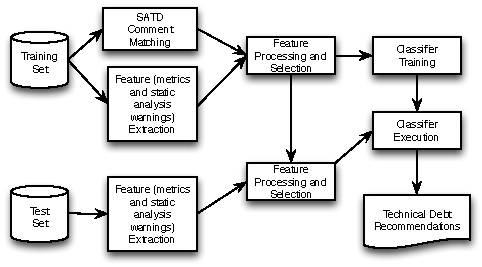
\includegraphics[width=\linewidth]{figs/approach.pdf}
	\caption{Proposed approach for recommending SATD with TEDIOUS.}
	\label{fig:approach}
	\vspace{-4mm}
\end{figure}

\ac{TEDIOUS} works as shown in Figure \ref{fig:approach}. Two datasets are required as inputs: the training set and the test set. The training set contains labeled data, which is source code from a project where technical debts are known and have been self-admitted through comments. The test set contains unlabeled data, which can be any source code under development or already released where \ac{TEDIOUS} can attempt to recommend where \ac{TD} should be self-admitted or where source code should be improved. \par 
	
For the training set, various kinds of metrics and static analysis warnings are extracted from methods in the source code as well as self-admitted technical debts in order to build an oracle to train the model. These labeled \ac{SATD} methods are essential for the machine learner since supervised learning is performed, meaning each method is labeled as true (containing a TD) or false. \par 

Once all the information is extracted, feature preprocessing and selection is applied. Multi-collinearity, a phenomenon occurring when two predictor variables are highly correlated, meaning that one can be linearly predicted by the other, is dealt with. Feature selection is applied to retain only the most relevant variables to train the predictors. Finally, rebalancing is performed to address the issue of the low number of positive examples, \textit{i.e.} \ac{SATD} methods. With the preprocessed features and the oracle now defined (each method is labeled as \ac{SATD} or not), the machine learners can be trained. \par 

In parallel, the test set is also being prepared. The same features are extracted from the source code but no \ac{SATD} matching is required since the data is unlabeled. \ac{SATD} are only required for the oracle, which is used for training the models. A similar feature filtering is applied, except for the rebalancing since it is only required on the labeled data. With both the test set and the previously trained classifiers, predictions can be made on the test set in order to recommend when to self-admit technical debts. \par

Each step of the process will be described in the following sections. Firstly, the features used will be detailed: source code metrics and warnings raised by static analysis tools. Secondly, the method employed to identify \ac{SATD} will be explained. Thirdly, the feature preprocessing tools will be summarized: multi-collinearity, feature selection and rebalancing. And finally, the training and application of the machine learning models will be explained.

\subsection{Features}

%3 pages

Three pieces of information extracted from the source code are necessary to accurately describe it: structural metrics, readability metrics and warnings raised by static analysis tools. There are reasons these specific features were chosen to describe the source code. Structural metrics are essential to capture symptoms of complex, heavily coupled and poorly designed code. These metrics explain the quality of the implementation and the software's design. Readability metrics quantify symptoms of poorly documented, hard to read and difficult to understand code. Warnings from static analysis tools are related to more specific bad coding choices rather than globally wrong code. They are issues which could lead to low maintainability and understandability of the code or which could potentially introduce defects in the future. In the following sections, these metrics and warnings are described more in depth.

\subsubsection{Source Code Metrics}

Nine source code metrics are extracted to characterize size, coupling and complexity. To define the size, metrics like \ac{LOC} or number of statements are calculated. For coupling, a metric such as the number of call sites is computed. For complexity, McCabe cyclomatic complexity \citep{mccabe1990reverse}, number of defined variables, number of expressions and number of identifiers are calculated. For readability, number of comments is an example of a metric used. It is important to know that not all comments are considered in the dataset. \ac{SATD} related comments are ignored in the empirical evaluation to avoid \ac{TEDIOUS} becoming a self-prophecy. Consequently, they are removed from the dataset. This issue will be covered later in the study design. \par

Firstly, to extract those source code metrics, an XML representation of the Java source code was generated using the tool srcML \citep{CollardKM03}. The computation of metrics was performed on this representation. It was also required to link comments to their related methods. Therefore, the rule used was that any comment directly preceding a method was assigned to it, as well as comments inside it. Comments could be a block of code or just single lines. This step is essential to be able to classify which method is a \ac{SATD} and which one is not. Some methods were excluded from our analysis because they did not fit the context of our research, namely getter and setter methods since they are irrelevant with design debts. To do so, we looked for method prefixes matching \emph{get} or \emph{set} and methods made up from more than a single line of code. When these two criteria were covered, the method was removed from the dataset. \par 

%Using  the {\em  srcML} tool, we processed each Java file, and stored the XML Java representation. We then used the Python ElementTree XML package to build the file level document object model; visiting the DOM and extracting methods along with  the attached comments and computing a set of structural metrics \Foutse{are these metrics different from those described in the approach section?}. We assigned to a method the method proceeding comments not separated from the method definition by any other statement. Then, as also described in Section \ref{sec:approach}, for each method we extracted source code structural metrics, the Buse and Weimer readability metric, and then we executed CheckStyle and PMD on each source code file. Finally, we mapped CheckStyle and PMD warnings onto methods, by knowing the line(s) in which a warning occurred and the line span of each method.

Secondly, to compute the code readability metric, we use the metric proposed by \citet{Buse:tse2010} and its related extraction tool, based on a machine learning approach. This metric is based on specific characteristics of the source code: indentation, line length, identifier length, comment density, and the use of keywords and operators. The tool was also designed using feedback from human annotators. They were asked to rate the readability of code snippets that were then used to classify snippets as "less" or "more" readable. A value between 0 and 1 is then computed based on these characteristics, 1 being the highest readability. The readability metric was considered relevant because, as mentioned by \citet{BavotaR16}, code readability is strongly correlated with the introduction of technical debts. Source code that is difficult to read is consequently difficult to maintain and understand \citep{Buse:tse2010}, and thus more likely to contain technical debts. Finally, here are the nine source-code metrics we extracted: \par

\begin{itemize}
\item \textit{LOC}: Number of lines of code in the body of a method. % (excluding comments).
\item \textit{Number of statements}: Number of occurrences of expression statements in a method. In case of local class definitions, the number of statements in the enclosing method is increased by the total number of statements of the local class.
\item \textit{Number of comments}: Number of single-line and multi-line comments in a method.
\item \textit{McCabe cyclomatic complexity}: Number of linearly independent paths of a method \citep{mccabe90}.
\item \textit{Number of passed parameters}: Number of parameters of a method.
\item \textit{Number of identifiers}: Number of unique identifiers in a method.
\item \textit{Number of call sites}: Number of locations in the code where zero or more arguments are passed to a method, or zero or more return values are received from the method.
\item \textit{Number of declarations}: Number of variable and class declarations in a method.
\item \textit{Number of expressions}: Number of expressions contained in a method.
\end{itemize}

\subsubsection{Warnings Raised by Static Analysis Tools}

Warnings raised by static analysis tools are essential to detect poor coding practices, which are also related to the introduction of technical debts. We cannot directly relate a flagged practice raised by an ASAT to a technical debt. However, we can wonder if multiple close warnings are justified and if they can be caused by the presence of a \ac{TD} in the source code. Having this hypothesis in mind, we used two popular static analysis tools, namely CheckStyle and PMD. Firstly, CheckStyle \citep{checkstyle} is widely used to check the adherence of code to standard practices and to detect pieces of code that are potentially smells. It performs an analysis based on a default configuration file, which can be modified at the discretion of users. For our research, the default configuration was used, containing code styles defined by Oracle and 43 checks. PMD \citep{pmd} main goal is to find common programming flaws such as unused objects, unnecessary catch blocks or incomprehensible naming. Similarly to CheckStyle, the default configuration was used, which contains 168 checks. Several reasons justify the choice of these two static analysis tools: they are commonly adopted by \ac{OSS} \citep{BellerBMZ16}, they provide a wide range of warnings related to code styles and programming practices, and they can be executed on source code statically. It is important to know that \ac{SATD} comments were removed when using these ASATs.

\subsection{Identification of Self-Admitted Technical Debt}

%0.5 page

As mentioned previously, the purpose of this thesis is not to propose a novel approach to detect \ac{SATD} using information from comments. Previous work has been completed aiming to address this issue by using pattern matching \citep{MaldonadoS15}, \citep{PotdarS14} or \ac{NLP} combined with machine learners \citep{maldonado17}. However, we still needed a dataset with methods tagged as design debt to train our machine learning models. \citet{maldonado17}, which worked on the \ac{NLP} approach, published a dataset of 10 open source projects annotated with methods tagged as technical debt or not. We used this dataset for our machine learning models where only the design debts were retained. \par

Some preprocessing had to be done on the dataset since it reported \ac{SATD} at file-level and not method-level. To link \ac{SATD} to methods, we matched the \ac{SATD} comment string to comments attached to methods. We used pattern matching in order to achieve this result, making sure that method comment strings completely matched \ac{SATD} comments before tagging the method as a technical debt.

\subsection{Feature Preprocessing}

%3 pages

Several features have been extracted from the source code, however, not all of them are relevant or necessary to train our models. Some clean up have to be done to reduce the size of the data input and improve the training phase. Multi-collinearity has to be dealt with, feature selection as to be applied and the training set has to be rebalanced.

\subsubsection{Multi-Collinearity}

We computed several features to characterize the source code of our software projects, however, some of them can be strongly correlated and can vary in the same way. Keeping these pairs of features would cause redundancy since they can be mutually and linearly predicted. That is why, when facing a pair of such features, we only keep the one that better correlates with the dependent variable (\ac{SATD} methods). The \emph{varclus} function in R, from the \emph{Hmisc} package, was used to help us achieve this preprocessing. This function performs a hierarchical cluster analysis of features to detect when two variable are positive based on similarity measures. It is mainly used to assess collinearity and redundancy, consequently resulting in data reduction. Hoeffding D statistic, squared Pearson or Spearman measures can be applied with \emph{varclus} to evaluate the correlation between variables. In this research, the Spearman's $\rho$ rank correlation measure was retained. To identify the problematic pairs using this coefficient, the cluster tree generated has to be cut at a particular level of $\rho^2$, which represents the correlation value. In our case, a value of $\rho^2=0.64$ was used since it corresponds to a strong correlation \citep{Cohen-1988}.

\subsubsection{Feature Selection and Normalization}

Some features will vary greatly or not at all between methods. These features are not useful to build a predictor because of their high degree of variance and they won't be impactful compared to all others available. The process of selecting only a relevant subset of all possible features is called \emph{feature selection}. Several reasons can justify going through this selection: to improve the prediction performance of machine learning models, to improve the speed and cost effectiveness of predictors, and to simplify models to better understand and interpret the underlying process behind the dataset generation \citep{guyon2003introduction}. \par 

The \emph{RemoveUseless} filter implemented in Weka \citep{hall2009weka} was used to perform feature selection. It looks for features that never vary or features that vary too much. For the latter, it looked for features that had a percentage of variance above a specific threshold, which was set up to 99\%. \par 

In addition to feature selection, the metrics were also normalized. Several projects were analyzed, all having significant differences in complexity and size characteristics. Therefore, normalization is necessary to reduce the effect of those differences during the training phase and to achieve good cross-project prediction performance. We will further discuss those characteristics of the dataset in the study definition section.

\subsubsection{Rebalancing}

To build performing predictors, a training set of quality must be fed to the machine learners. One important aspect is to have a balanced dataset, which means having as much as possible an equal number of positive and negative examples. In our context, this means as many \ac{SATD} tagged methods as correct methods. This is a serious problem for us since the vast majority of methods are not technical debts (this will be discussed more in depth in the next section), only a minority contains \ac{SATD}. 

There are two ways to address this issue: under-sample the majority class (methods with no \ac{SATD}) or over-sample the minority class (\ac{SATD} tagged methods). Since the training set is so highly unbalanced, which means the number of instances of the minority class is excessively small, the second option was favored. In fact, under-sampling would result in a very small training set. 

To apply over-sampling, artificial instances of \ac{SATD} methods must be generated from the existing ones. To do so, Weka provides a tool to perform over-sampling, called \ac{SMOTE} \citep{chawla2002smote}, which combines under-sampling the majority class and over-sampling the minority class to achieve improved classifier performance.

\subsection{Building and Applying Machine Learning Models}

%0.5 page
 We extracted various metrics, we identified \ac{SATD} methods and we performed the preprocessing of features, the only remaining step is building and applying the machine learning models. Two sets are required: the training set and testing set. The training set contains the methods with their corresponding features and an additional variable to tag them as positive or negative (\ac{SATD} or not). This set is used to build the models. The testing set contains the same methods with their corresponding features, but not the variable tagging the methods because we want to test the prediction performance on a blank dataset. We experimented with five types of machine learners in Weka \citep{hall2009weka}: Decision Trees (J48), Bayesian classifiers, Random Forests, Random Trees, and Bagging with Decision Trees. Only default configurations were used, however, further work could be done by trying to optimize these configurations. Here is a little overview of each algorithm: \par 

\begin{itemize}
\item \textit{Decision trees}, namely J48, implement the standard C4.5 algorithm using the concept of information entropy \citep{Quinlan1993}.
\item \textit{Bayesian classifiers} apply the Bayes' theorem to classify observations, assuming strong independence between features. More specifically, we use BayesNet in Weka, which is the base class for Bayes Network classifiers. It provides data structures and facilities common to learning algorithms K2 and B.
\item \textit{Random forests} average multiple decision trees trained on different parts of a same training set. The goal is to reduce the variance of classifications and the risk of overfitting the training set \citep{Breiman2001}.
\item \textit{Random trees} build decision trees considering a number of randomly chosen attributes at each node.
\item \textit{Bagging} combines multiple classifiers (decision trees in our case) built on random samples of the training set \citep{Breiman1996}. It was designed to improve the stability and accuracy of machine learning algorithms, to reduce the variance and to avoid overfitting.
\end{itemize}

 
\begin{landscape}
 \begin{figure}[t]
 	\centering
 	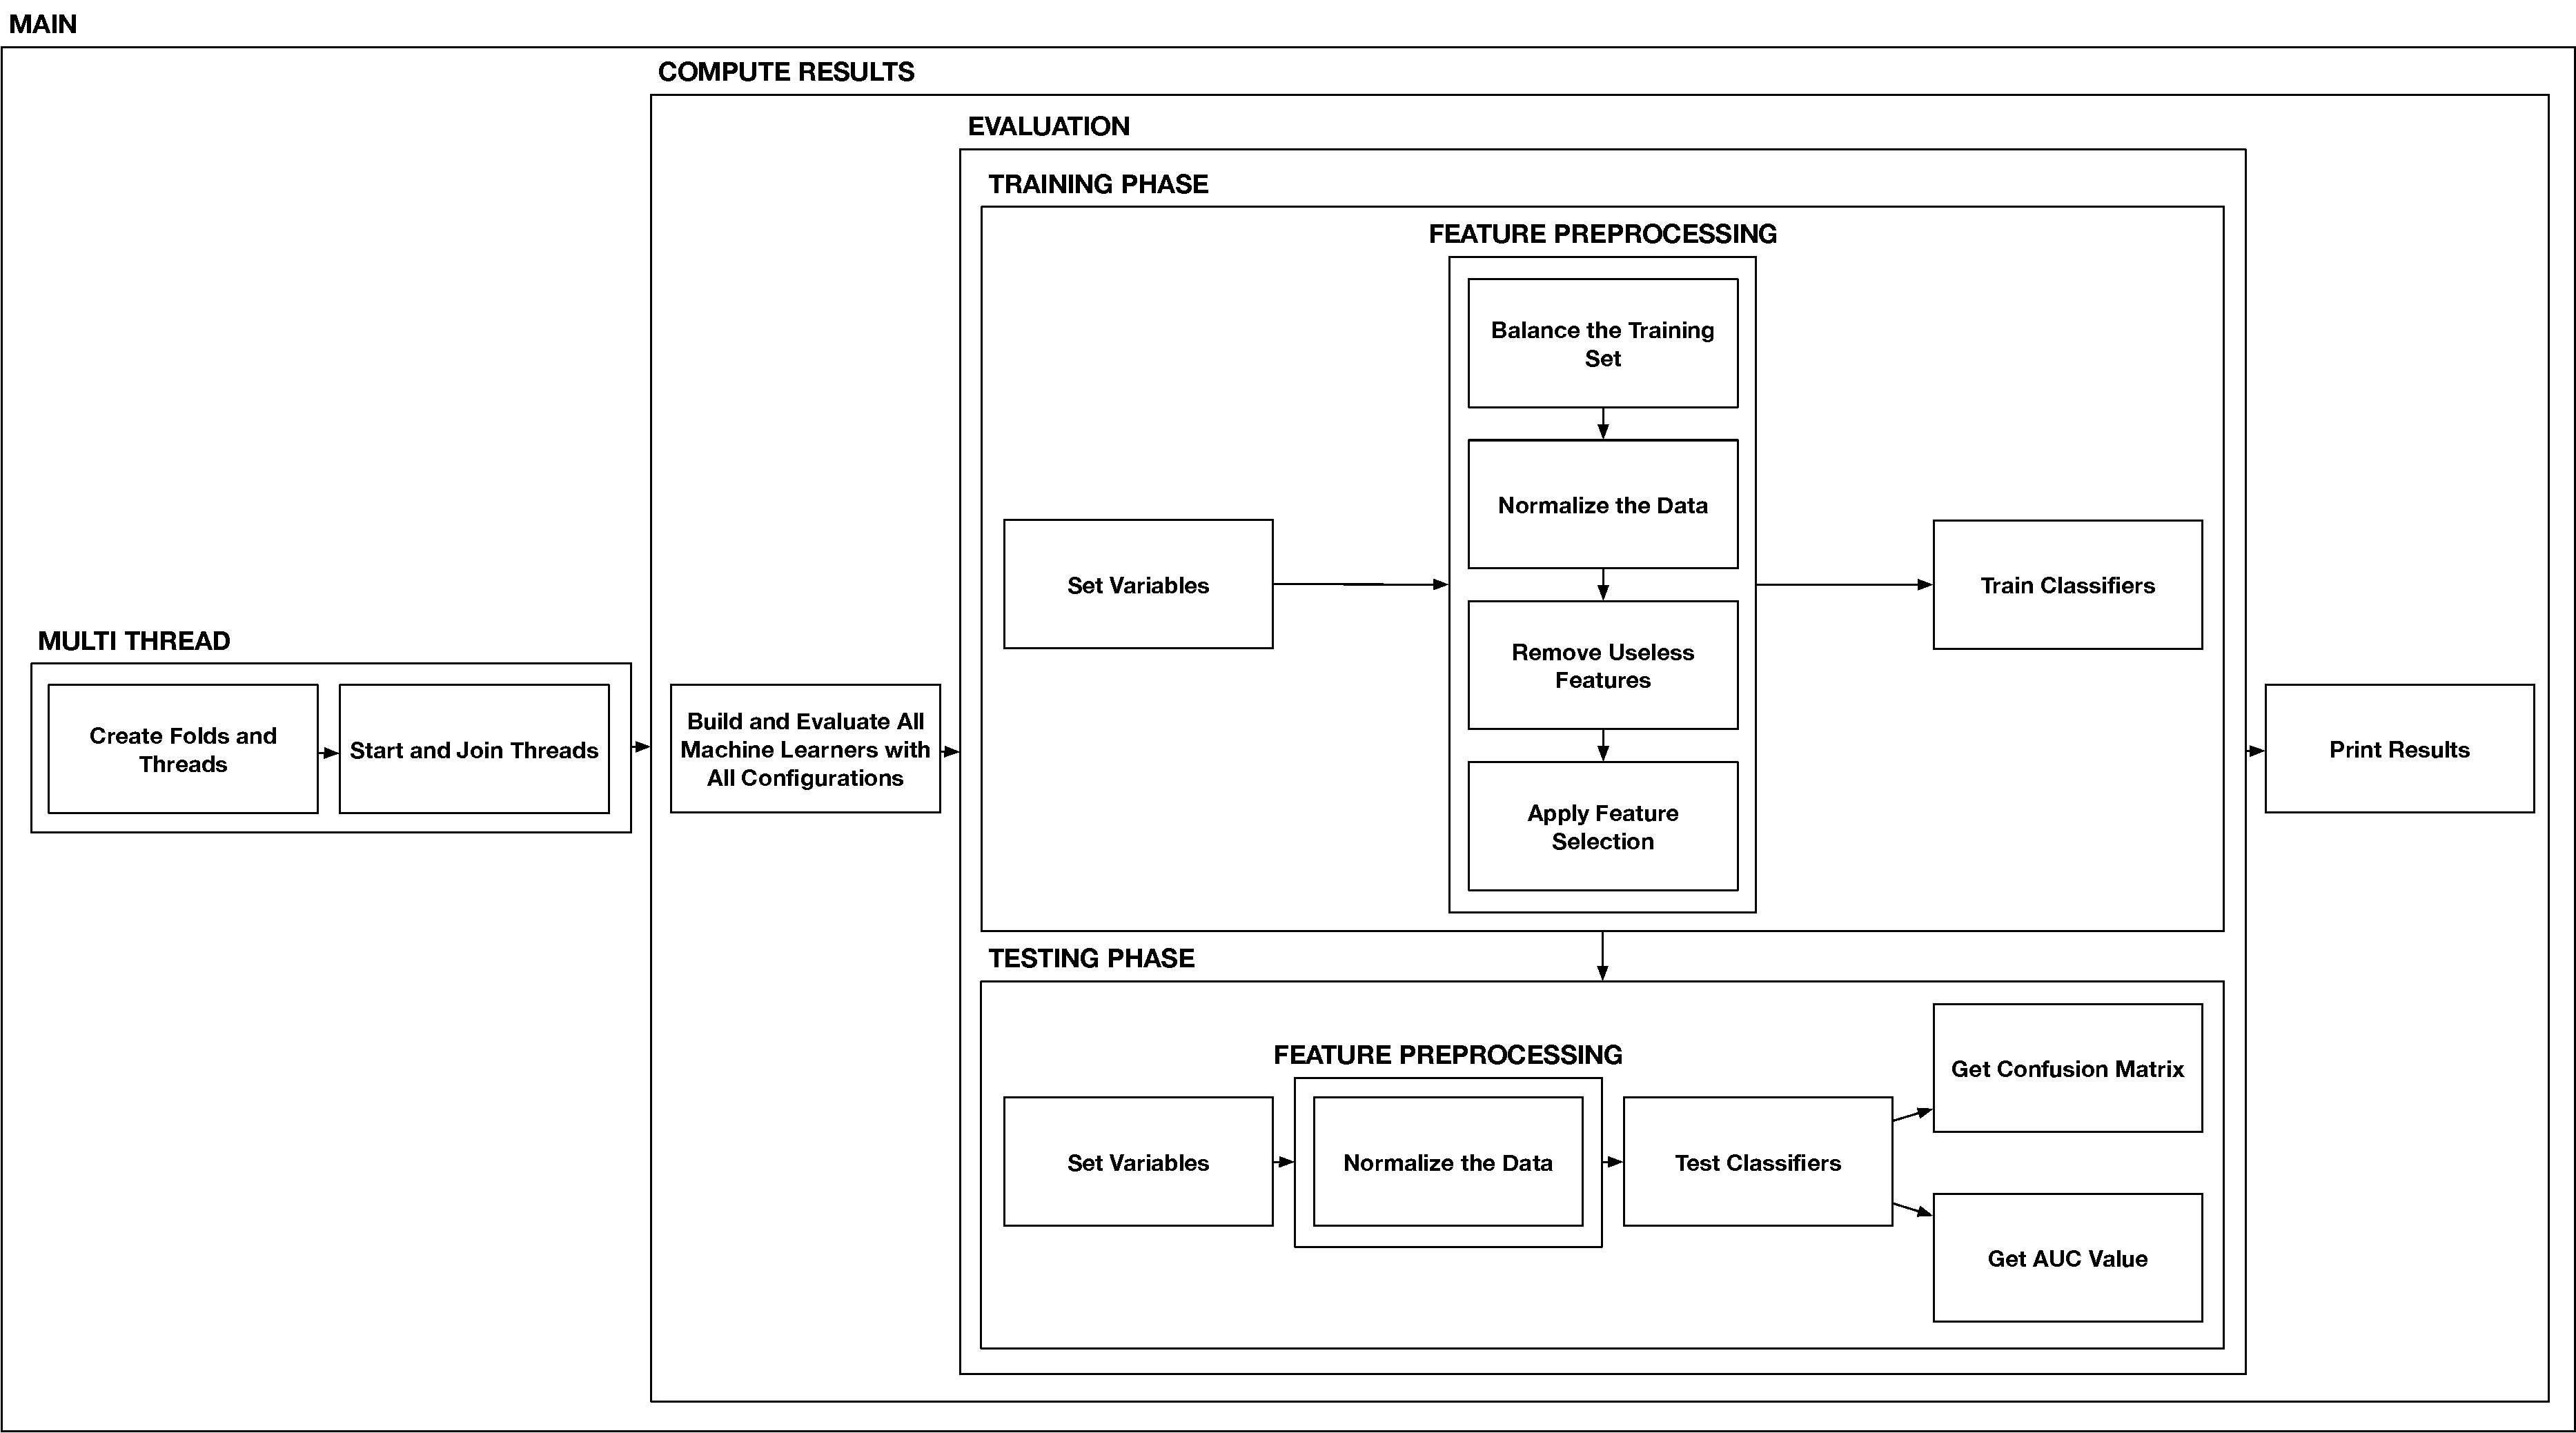
\includegraphics[width=\linewidth]{figs/MachineLearning.pdf}
 	\caption{Process for building and applying machine learners.}
 	\label{fig:MLProcess}
 	\vspace{-4mm}
 \end{figure}
\end{landscape}
 
 %\textbf{SHOW IMAGE OF PSEUDOCODE AND EXPLAIN IT. VOIR LE ECLIPSE PROJECT QUE FIORELLA A ENVOYE.} 
 
 Figure \ref{fig:MLProcess} provides an overview of the machine learning process. To increase the training speed, several threads are created. For the 10-fold cross-validation inter-project analysis, one thread is started for each fold, which was generated beforehand for each software system. Actions in the evaluation phase are performed simultaneously on each thread and the computation is finished once all of them are finished. All possible combinations of machine learners and configurations are used for training and testing on each fold. We have 5 different types of machine learners, the possibility of balancing the training set, and the possibility of applying feature selection, for a total of 20 possible predictors per fold. \par
 
 The evaluation phase consists of a training and testing phase. In the training phase, the variables to predict are initialized, \emph{i.e} \ac{SATD} methods, and feature preprocessing is applied. This means that the training set can be balanced or not, data is normalized, useless features are removed and feature selection can be applied or not. Afterwards, the classifiers are trained. In the testing phase, the variables to predict are initialized again. As for the feature preprocessing, only data normalization is performed. The classifiers are tested and then the confusion matrix and the AUC value are computed. Finally, results are printed to perform a deeper analysis.
 
\section{Study Definition}

%0.5 page

The goal of this thesis is to assess the prediction performance of our machine learning based approach in recommending technical debts to self-admit. The focus is to enhance source code quality, more specifically its maintainability and understandability, by keeping track of technical debts which can be corrected in the future. The perspective of this thesis is to be able to suggest to developers when to admit technical debts. Globally, we aim at addressing three research questions:

\begin{itemize}
	\item \textbf{RQ1}: How does \ac{TEDIOUS} work for recommending \ac{SATD} within project?
	\item \textbf{RQ2}: How does \ac{TEDIOUS} work for recommending \ac{SATD} across projects?
	\item \textbf{RQ3}: How would a method-level smell detector compare with \ac{TEDIOUS}?
\end{itemize}

\begin{landscape}
\begin{table*}[t]
	\caption{Characteristics of the studied projects.}
	\label{tab:projects}
	\centering
		\begin{adjustbox}{center}
			\begin{tabular}{l r | r r r r | r | r r | r}
				\hline
				\multirow{2}{*}{Project} & \multirow{2}{*}{Release} &\multicolumn{4}{c|}{Number of} &\multicolumn{1}{c|}{Number of Comments}
				&\multicolumn{2}{c|}{Number of Design SATD} & \% of Methods\\
				&& Files& Classes& Methods& Comments                      & $\in$ Methods& $\notin$ Methods & $\in$ Methods & with design SATD\\
				\hline
				Ant&1.7.0 & 1,113 & 1,575 & 11,052 & 20,325               & 13,359        &  1 & 57 & 0.5\% \\
				ArgoUML&0.34& 1,922 & 2,579 & 14,346 & 64,393       &  17,722       & 203 & 425  & 2\%\\
				Columba&1.4& 1,549 & 1,884 & 7,035 & 33,415           & 10,305        & 8 & 418 & 5\%  \\
				Hibernate&3.3.2 GA & 2,129 & 2,529 & 17,405 & 15,901 & 9,073        & 21  &  377  &  2\%\\
				jEdit & 4.2 & 394 & 889 & 4,785 & 15,468                     &10,894         & 6  & 77  & 2\% \\
				jFreeChart&1.0.19 & 1,017 & 1,091 & 10,343 & 22,827  & 15,412       &  4  & 1,881  & 18\%\\
				jMeter&2.1& 1,048 & 1,328 & 8,680 & 19,721                &  12,672      & 95 &  424 & 5\%  \\
				jRuby&1.4.0 & 970 & 2,063 & 14,163 & 10,599               & 7,809        & 16   & 275  &  2\%\\
				Squirrel&3.0.3 & 2,325 & 4,123 & 16,648 & 25,216         & 15,574      &35  & 173  & 1\%\\
				\hline
			\end{tabular}
		\end{adjustbox}
		\vspace{-4mm}
\end{table*}
\end{landscape}

\subsection{Dataset}

%2 pages

To evaluate our approach, we used a dataset that was already analyzed to find \ac{SATD} methods \citep{maldonado17}. Those methods were detected using a NLP approach, and then manually validated and classified. The dataset contains 10 open source projects, however, we only used 9 of them since we could not download the specific version of EMF. Table \ref{tab:projects} summarizes the characteristics of all studied projects. It provides information on project releases; number of files, classes, methods and comments in projects; number of comments in methods; number of design \ac{SATD} in methods and in classes; and percentage of methods with design \ac{SATD}. \par

Some differences were observed with the characteristics extracted from the original paper \citep{maldonado17}, concerning the number of classes, methods and comments. Several reasons can explain these disparities: usage of different extraction tooling, tools characteristics and processing. For example, we considered each comment as a single entity, whereas \citet{maldonado17} regrouped successive line comments. Additionally, we did not establish a separation between classes and their inner classes, and we considered interfaces as classes. Methods related to inner classes were associated to its container. However, these differences are not an issue for our research since they concern classes and our approach is method-level based. Additionally, some files from \citet{maldonado17} analysis could have been left aside because of their absence of comments. \par 

We observe some interesting facts when looking at Table \ref{tab:projects}. As explained previously, we clearly see the prevalence of method-related \ac{SATD} compared to class-level \ac{SATD}. They are at least 2 times more common for \textsc{ArgoUML}, which contains about half of all the class-level \ac{TD} in the dataset, and can be up to 470 times more common for \textsc{jFreeChart} where only 4 of the 1,885 design \ac{SATD} are at class-level. Globally, we are around 10 times more likely to encounter a method-level design technical debt in our dataset than class-level. We also observe that the dataset is highly unbalanced between \ac{SATD} prone and non-\ac{SATD} prone methods. \textsc{jFreeChart} provides a decent ratio with 18\% of methods containing a design technical debt, but all other projects have 5\% or less of their methods containing design debts. To put this into perspective, out of the 11,052 methods in \textsc{Ant}, only 57 are \ac{SATD} prone. For \textsc{jEdit}, only 77 instances out of 4,785 are proned to contain a \ac{SATD}. Unsurprisingly, as we will discuss in the analysis of study results, these two projects achieved the lowest performance values. \par 

The replication package provided by \citet{maldonado17} contains information on \ac{SATD} at class-level and not method-level. The issue is that we need to assign \ac{SATD} at method-level to build our oracle. To do so, we performed pattern matching between known \ac{SATD} comments from the replication package and comments attached to methods in the 9 software projects. The other cases are: if a comment is matched inside a class but not a method, it is attached to the class, and if it is matched outside of a class, it is attached to the file. These class-level and file-level technical debts are not considered in our research, which is not a big issue since they represent a minority of all design debts.

\subsection{Analysis Method}

%3.5 pages

For \textbf{RQ1}, we want to know how \ac{TEDIOUS} works for recommending \ac{SATD} within project. A 10-fold cross validation was performed on each project. In other terms, the dataset of a single project is divided into 10 folds, the machine learner is trained on 9 of them and tested on the remaining one, until all 10 configurations are processed in order to limit the effect of randomness. The performance values are averaged over the 10 iterations to obtain the most representative picture. For \textbf{RQ2}, we want to know how our approach works for recommending \ac{SATD} across projects. The process is similar to \textbf{RQ1}, but instead we train on 8 projects and test on the remaining one, until all 9 possible combinations are executed. \par 

Standard performance metrics to evaluate automated classification were computed to analyze our approach: precision, recall and $F_{1}$ score. These metrics were computed for the \ac{SATD} category. \par 

\ac{Pr} is the percentage of relevant instances of methods predicted as \ac{SATD} among all retrieved instances. \ac{TP} and \ac{FP} are respectively the number of true positives, correct methods predicted as \ac{SATD}, and false positives, incorrect methods predicted as \ac{SATD}.

\[
Pr=\frac{TP}{TP+FP}
\]

\ac{Rc} is the percentage of relevant instances of \ac{SATD} methods that have been retrieved over all relevant instances. \ac{FN} is the number of false negatives, incorrect methods predicted as non-\ac{SATD}.

\[
Rc=\frac{TP}{TP+FN}
\]

The $F_{1}$ score is the harmonic mean between precision and recall, which provides a single measurement to evaluate a system.

\[
F_1=2 \cdot \frac{PR \cdot RC}{PR + RC}
\]

The previous metrics are specific to the \ac{SATD} class, which means true negatives \ac{TN}, correct methods predicted as non-\ac{SATD}, are not considered yet in the performance evaluation. Consequently, other metrics are required to complement the analysis: accuracy, Matthews Correlation Coefficient (MCC) \citep{matthews1975comparison}, and the Area Under the Curve (AUC) of the Receiving Operating Characteristics (ROC). \par 

\ac{Acc} is the total number of methods correctly predicted, whether it is containing a \ac{SATD} or not, among all the methods analyzed.

\[
Acc=\frac{TP+TN}{TP+TN+FP+FN}
\]

The \ac{MCC} is a metric used in machine learning to evaluate the quality of a two-class classifier. It is especially useful when the dataset is unbalanced \citep{matthews1975comparison}. Values vary between -1 for a completely wrong classifier and 1 for a perfect classifier. 

\[
MCC=\frac{TP \cdot TN-FP \cdot FN}{\sqrt{(TP+FP)(FN+TN)(FP+TN)(TP+FN)}}
\]

The \ac{ROC} curve is created by plotting the true positive rate against the false positive rate at various classifier thresholds. The \ac{AUC} is the area under the ROC curve, it provides a value to evaluate the quality of the classifier. A value of AUC=0.5 refers to a random classifier and the higher the value, the better the classifier.

To have a good idea of the performance of each machine learner, each of the previous metrics have to be considered in the evaluation. We want a balance between precision and recall because we want as much as possible to detect real technical debts and all of them. We cannot only use $F_{1}$ score because we want to take into account the effect of chance on predictions made. That is why we also computed the MCC and AUC values.

In addition to these performance indicators, we also consider the importance of each features during the training of the predictors. We used a technique implemented in Weka for Random Forests named \ac{MDI} \citep{louppe2013understanding}, which measures the importance of variables on randomized decision trees.

For \textbf{RQ3}, we want to compare \ac{TEDIOUS} with a popular method-level smell detector (DECOR) \citep{moha2010decor} in classifying as technical debt methods labeled as \ac{SATD}. DECOR can detect a large amount of smells, but most of them are at class-level, which are not relevant to the level at which \ac{TEDIOUS} works. Instead of using all of them, we narrowed our analysis to two method-level smells, \textit{Long Method} and \textit{Long Parameter List}. 

To identify a Long Method smell, DECOR follows the rule {\em LOC}$>th_1$ where $>th_1$ is a threshold for the LOC. To identify a Long Parameter List smell, DECOR follows the rule {\em ParNbr}$>th_2$ where $>th_2$ is a threshold for the number of parameters. Various thresholds for LOC and ParNbr were considered in our research, between percentiles 0.5 and 0.95, as well as the default thresholds, more specifically percentile 0.75 for LOC and outlier (third quartile $+ 1.5 \cdot IQR$ (interquartile range)) for ParNbr.

To finish, we performed a qualitative analysis on false positives and false negatives examples we obtained when evaluating our predictors. Its purpose is to complement our quantitative analysis and discuss the limitations of our approach in recommending \ac{TD} with real examples.
























